\section{IEC funksjonsblokker} \label{IEC Seksjon}
\thispagestyle{fancy}

Vi gjorde eit utval av moglege funksjonsblokktemplat basert på dei komponentane vi identifiserte i reinseanlegget.
For å lage eit robust program valde vi å fokusere på to inngangsfunksjonar, \gls{MA}, \gls{MB}, og to utgangsfunksjonar \gls{SBE}, \gls{SBV},
som måtte programmerast frå grunn. 

Funksjonsblokktemplata inneholdt avanasert funksjonalitet som vi visste ville ta lang til å programmere.
Sjølv om ikkje all denne funksjonaliteten var naudsynt for reinseanlegget,
valde vi likevell å programmere alt, ettersom blokkene gir potensiell meirverdi i mogleg utvidning og eventuell bruk i andre styresystem.
Det gav oss også ein tydleg retning å arbeide mot og vi visste at blokka ville dekke alle aktuelle behov.

\gls{IEC} har sentrale begrep som vi ønskjer å utdjupe nærmare. Grunna mangel på gode norske begrep
og for å forhindre forvirring velger vi å beskrive begrepa slik dei er skildra i normen \citep{IECGlossery}

\begin{itemize}
    \item \textbf{Lock:} Action overruling any other signal while being true
    \item \textbf{Force:} Action overruling any other signal                        
    \item \textbf{Disable transition:} Transistion high/low function not avaliable  
    \item \textbf{Blocking:} Prevention of certain functions or operations          
    \item \textbf{Suppression:} Disable alarm annunciation as well as any associated automatic actions
\end{itemize}
Det er også andre genrelle forkortingar som er viktige i skildring av desse blokkene.
\begin{figure}[htbp]
    \centering
    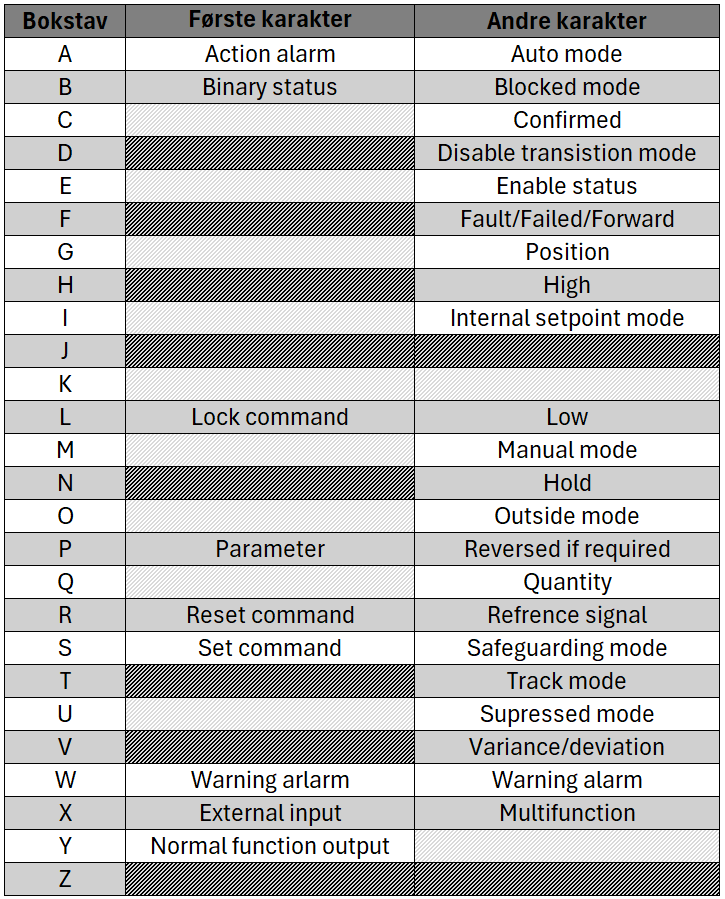
\includegraphics[scale=0.33]{Figurar/IEC bokstavmatrise.png}
    \caption{Bokstavmatrise basert på Table A.1 i \gls{IEC} \gls{PAS} 63131:2017 \citep{A1}}\label{fig:SBE tilstandsmaskin}
\end{figure}

\newpage

\subsection{Monitor Binary}
Inngangsfunksjon \gls{MB} blir nytta til automatisk overvaking, alarmhandtering, framvising og låsing av binære prosessvariablar \citep{IEC-63131}.
Funksjonsblokka er nytta i programmet for å overvake alle digitale inngangar t.d. pressostat og nivåvipper.

\gls{MB} mottar binær verdi på X og returnerer verdi på Y. \newline
Denne utgangsverdien har moglegheit for tidsforseinking, invertering, låsning, ``blocking'' og ``suppression'' via ``force'' inngangsvariablar og parameter.

Blokka har tre statusvariablar som indikerer modus og område (BU, BB, BX), ein utgang for indikasjon av feil (YF) med moglegheit for ``suppression''
og ein inngang (RX) for reset av eventuell låst verdi. \newline 

\begin{figure}[htbp]
    \centering
    \begin{subfigure}[b]{1\textwidth}
        \centering
        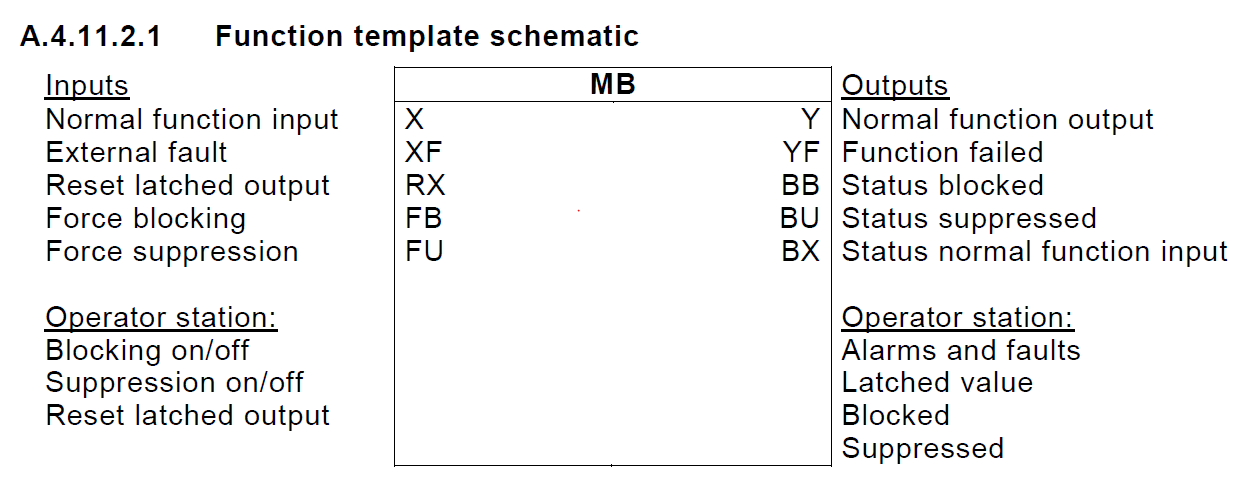
\includegraphics[width=0.7\textwidth]{Bilder/MBBlokkIEC.png}
        \caption{\gls{IEC} \gls{PAS} 63131:2017 \citep{MB}}\label{fig:Monitor Binary blokk IEC}
    \end{subfigure}
    \hfill
    \begin{subfigure}[b]{1\textwidth}
        \centering
        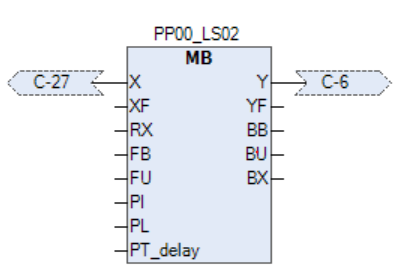
\includegraphics[width=0.5\textwidth]{Bilder/MBBlokkIProgrammet.png}
        \caption{MB nytta i programmet}\label{fig:Monitor Binary blokk i programmet}
    \end{subfigure}
    \caption{Monitor Binary}\label{fig:Monitor Binary}
\end{figure}

Meir informasjon om blokka, inngangar, utgangar, og parameter er tilgjengeleg i vedlegg. (Vedlegg C.1)

\newpage

\subsection{Monitor Analogue}
Inngangsfunksjon \gls{MA} er nytta for skalering, visning, overvaking og alarmhandtering av
analoge prosess og kontrollvariablar \citep{IEC-63131}.
Funksjonsblokka er nytta for å overvake analoge trykknivågivarar 
og å skalere og vise desse som ein fyllingsgrad i prosent.

\gls{MA} hentar rå analog verdi på X og returnerer verdi på Y.
Denne utgangsverdien blir skalert basert på parameter og har hysterese og dødband tilgjengeleg.

Hysterese og dødband definerer områder rundt eit gitt setpunkt der systemet 
ikkje endrar tilstand eller reagerer på små variasjonar.
Dette gjer at systemet unngår hyppige vekslingar og unødvendige justeringar.

Funksjonsblokka har to forvarsel (WH og WL) og to handlingar med alarm (AHH og ALL).
Det er moglegheit for tidsforsinking, ``blocking'' og ``suppression'' av desse via ``force'' inngangsvariablar og parameter.

Blokka har fem statusvariablar som indikerer modus og område (BU, BB, BHH, BLL, BBLL, BBHH), ein utgang for indikasjon av feil (YF)
og fire hendingar (BXHH, BXH, BXLL, BXL) utan ``blocking'' og ``suppression'' som nyttast for styring.

Grenser på varsling og hendigar er justerbare via parameter.

\begin{figure}[htbp]
    \centering
    \begin{subfigure}[b]{0.49\textwidth}
        \centering
        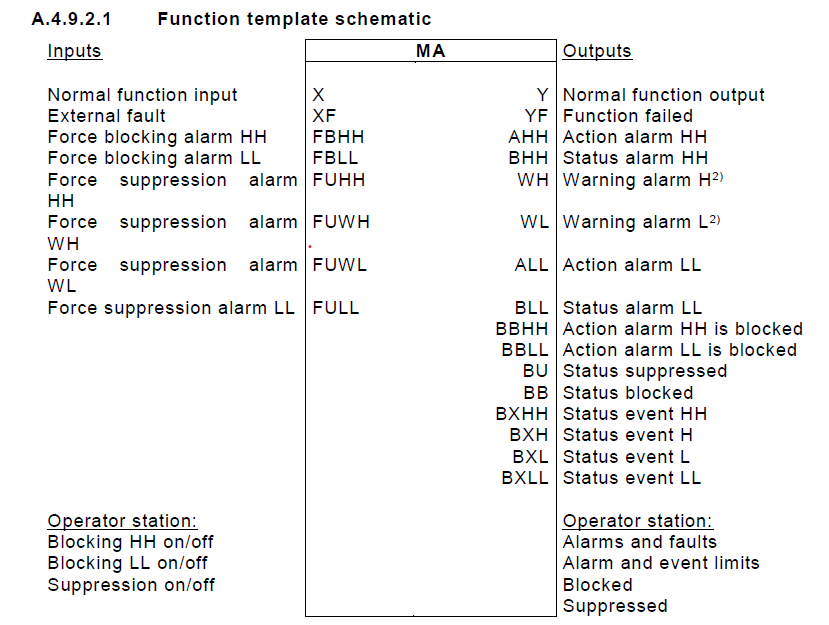
\includegraphics[width=1\textwidth]{Bilder/MABlokkIEC.png}
        \caption{\gls{IEC} \gls{PAS} 63131:2017 \citep{MA}}\label{fig:Monitor Analogue blokk IEC}
    \end{subfigure}
    \hfill
    \begin{subfigure}[b]{0.49\textwidth}
        \centering
        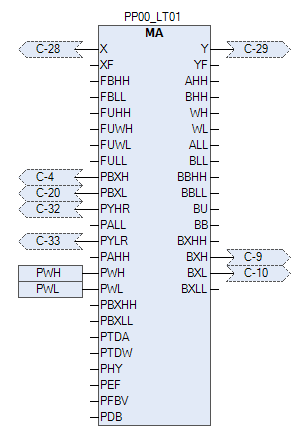
\includegraphics[width=0.7\textwidth]{Bilder/MABlokkIProgrammet.png}
        \caption{MA nytta i programmet}\label{fig:Monitor Analogue blokk i programmet}
    \end{subfigure}
    \caption{Monitor Analogue}\label{fig:Monitor Analogue}
\end{figure}

Meir informasjon om blokka, inngangar, utgangar, og parameter er tilgjengeleg i vedlegg. (Vedlegg C.2)

\newpage

\subsection{Switch Binary Eletrical} 

Utgangsfunksjon \gls{SBE} blir nytta for binærkontroll (av/på) av straumningselement for elektrisitet, varme eller væske. 
Den kontrollerte komponenten kan vere t.d. motor, pumpe, varmeelement, vifte \citep{IEC-63131}. \newline
Funksjonsblokka er nytta til å styre motorar, pumper og blåserar. (Vedlegg C.3)

Funksjonsblokka har tre modus, auto, manuell og lokal. Lokal betyr lokal HMI eller direktekøyring.
\gls{SBE} hentar start/stopp signal på
\begin{enumerate}
    \item \textbf{Auto:}        XH og XL  
    \item \textbf{Manuell:}     HMI
    \item \textbf{Lokal:}       XOH og XOL
\end{enumerate}
Aktiveringssignal er tilgjengeleg via inngang XE. \newline
Blokka gir tilbake køyrsignal på Y og via pulsmodulerte utgangar YH og YL.

\gls{SBE} inneheld ei tilstatandsmaskin med fire funksjonstilstandar. 
\begin{enumerate}
    \item \textbf{Høg:}                 Komponent køyrer
    \item \textbf{Lav:}                 Komponent stoppa
    \item \textbf{Transisjon mot lav:}  Fått stoppsignal
    \item \textbf{Transisjon mot høg:}  Fått køyreesignal.
\end{enumerate}

I transisjonstilstand ventar blokka på eksternt tilbakemelding (XGH) 
og sett tilstanden til høg/lav etter at korrekt tilbakemelding er mottatt.
Dette vises også via to statusvariablar (BCL, BCH)

Blokka har sju andre statusvariablar som indikerer modus og område (BA, BO, BS, BB, BU, BXH, BXL) og
ein utgang for indikasjon av feil (YF) med tilhøyrande heiltallsverdi (YFI) som indikerer feiltype. \newline
Feilstatus har moglegheit for ``suppression''.

Blokka har fire signal for høg/lav tvangskøyring, der ``lock'' endrar modus til maneull (LSH, LSL) og ``force'' gjer ikkje (FSL, FSH)
og to signal for høg/ lav ``force disable transition'' (FDH, FDL).
Desse signala har moglegheit for ``blocking''.

\newpage

\begin{figure}[htbp]
    \centering
    \begin{subfigure}[b]{0.46\textwidth}
        \centering
        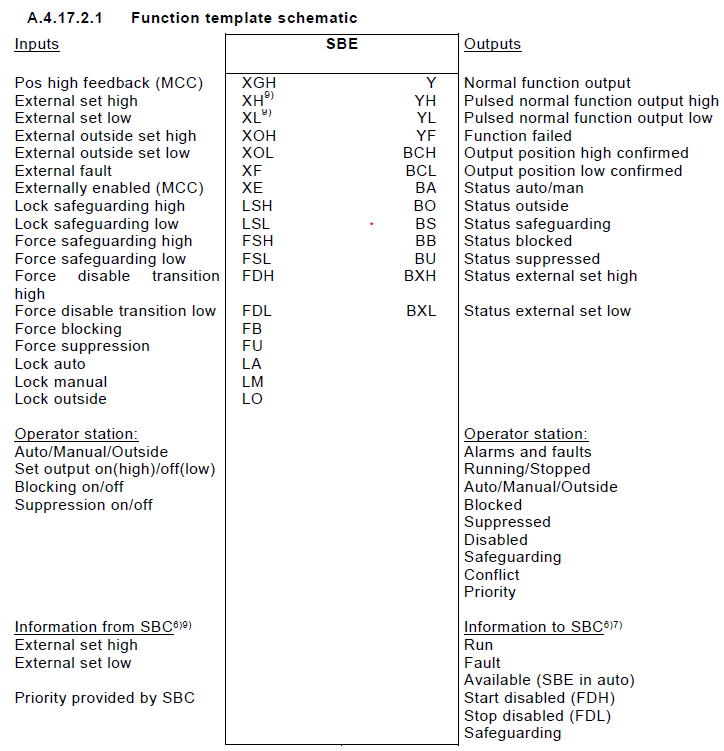
\includegraphics[width=1\textwidth]{Bilder/SBEBlokkIEC.png}
        \caption{\gls{IEC} \gls{PAS} 63131:2017 \citep{SBE}}\label{fig:Switch Binary Electrical blokk IEC}
    \end{subfigure}
    \hfill
    \begin{subfigure}[b]{0.46\textwidth}
        \centering
        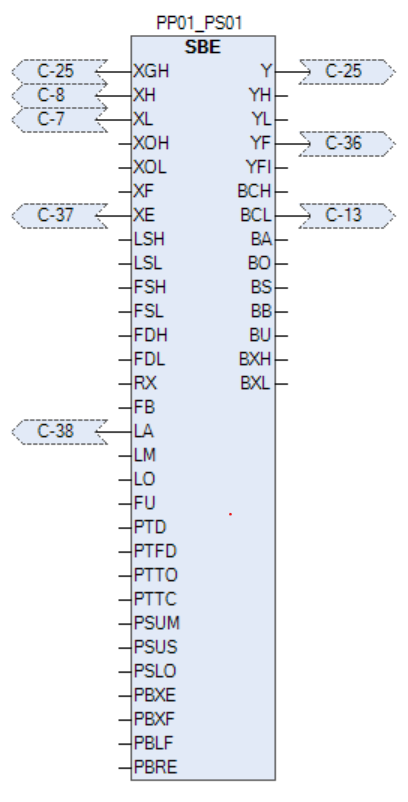
\includegraphics[width=0.5\textwidth]{Bilder/SBEBlokkIProgrammet.png}
        \caption{SBE nytta i programmet}\label{fig:Switch Binary Electrical blokk i programmet}
    \end{subfigure}
    \caption{Switch Binary Electrical}\label{fig:Switch Binary Electrical}
\end{figure} 
\begin{figure}[htbp]
    \centering
    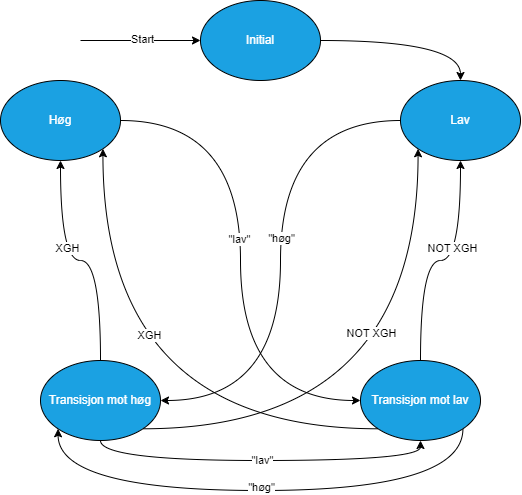
\includegraphics[scale=0.45]{Figurar/SBE.drawio.png}
    \caption{Prinsippskisse SBE tilstandsmaskin standard parameteroppsett}\label{fig:SBE tilstandsmaskin}
\end{figure}
Meir informasjon om blokka, inngangar, utgangar, og parameter er tilgjengeleg i vedlegg. (Vedlegg C.3)
\newpage
\subsection{Switch Binary Valve}

Utgangsfunksjon \gls{SBV} skal nyttast til binær (av/på) kontroll av eit straumningselement ved å endra straumen av medium (varme eller væske). 
Typisk komponentar som styrast er bl.a. ventilar og spjeld \citep{IEC-63131}.
Funksjonsblokka er i nytta til å styre ventilar.

Samenlika med \gls{SBE} har \gls{SBV} har tre modus, auto, manuell og lokal som nyttar inngagnar med same namn.
\gls{SBV} hentar opne/stenge signal på
\begin{enumerate}
    \item \textbf{Auto:}        XH og XL  
    \item \textbf{Manuell:}     HMI
    \item \textbf{Lokal:}       XOH og XOL
\end{enumerate}
Blokka gir tilbake signal på Y og via pulsmodulerte utgangar YH og YL.

\gls{SBV} inneheld ei tilstatandsmaskin med fire funksjonstilstandar. 
\begin{enumerate}
    \item \textbf{Høg:}                 Komponent open
    \item \textbf{Lav:}                 Komponent stengd
    \item \textbf{Transisjon mot lav:}  Fått stengesignal
    \item \textbf{Transisjon mot høg:}  Fått opnesignal.
\end{enumerate}

I transisjonstilstand ventar blokka på eksternt tilbakemelding (XGH, XGL) 
og sett tilstanden til høg/lav etter at korrekt tilbakemelding er mottatt.
Dette vises også via to statusvariablar (BCL, BCH)

Blokka har fem andre statusvariablar som indikerer modus og område (BA, BO, BS, BB, BU) og
ein utgang for indikasjon av feil (YF) med tilhøyrande heiltallsverdi (YFI) som indikerer feiltype. \newline
Feilstatus har moglegheit for ``suppression''.

Blokka har fire signal for høg/lav tvangskøyring, der ``lock'' endrar modus til maneull (LSH, LSL) og ``force'' gjer ikkje (FSL, FSH)
og to signal for høg/ lav ``force disable transition'' (FDH, FDL).
Desse signala har moglegheit for ``blocking''.

\newpage

\begin{figure}[htbp]
    \centering
    \begin{subfigure}[b]{0.45\textwidth}
        \centering
        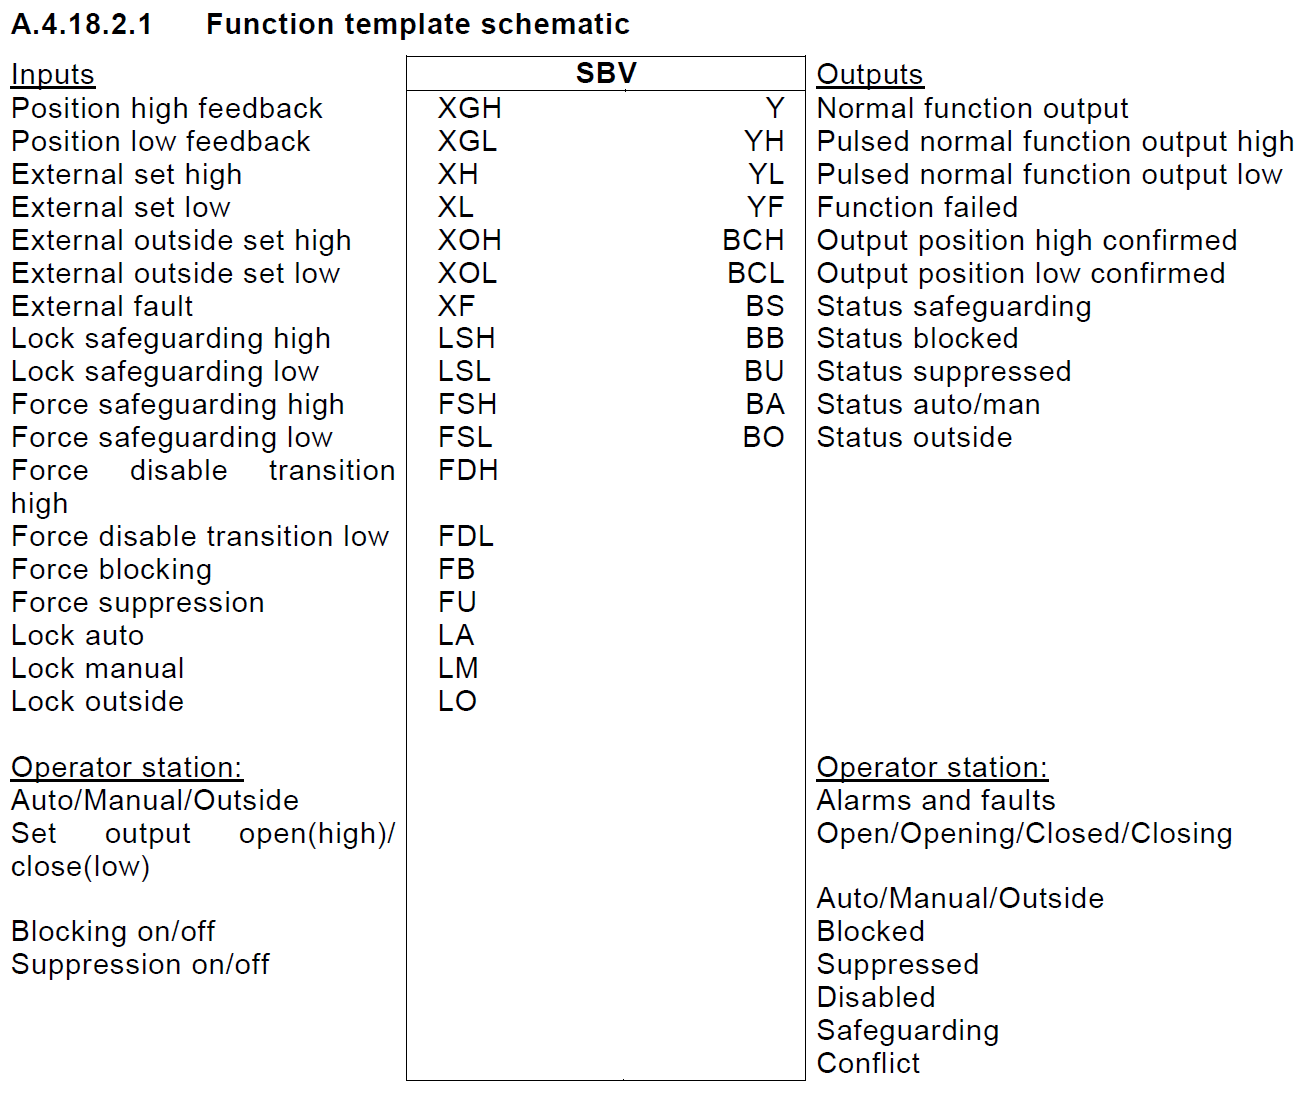
\includegraphics[width=1\textwidth]{Bilder/SBVBlokkIEC.png}
        \caption{\gls{IEC} \gls{PAS} 63131:2017 \citep{SBV}}\label{fig:Switch Binary Valve blokk IEC}
    \end{subfigure}
    \hfill
    \begin{subfigure}[b]{0.45\textwidth}
        \centering
        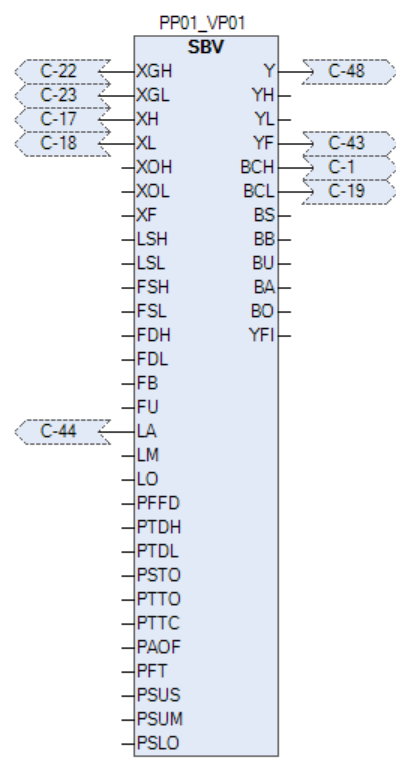
\includegraphics[width=0.5\textwidth]{Bilder/SBVBlokkIProgrammet.png}
        \caption{SBV nytta i programmet}\label{fig:Switch Binary Valve blokk i programmet}
    \end{subfigure}
    \caption{Switch Binary Valve}\label{fig:Switch Binary Valve}
\end{figure}
\begin{figure}[htbp]
    \centering
    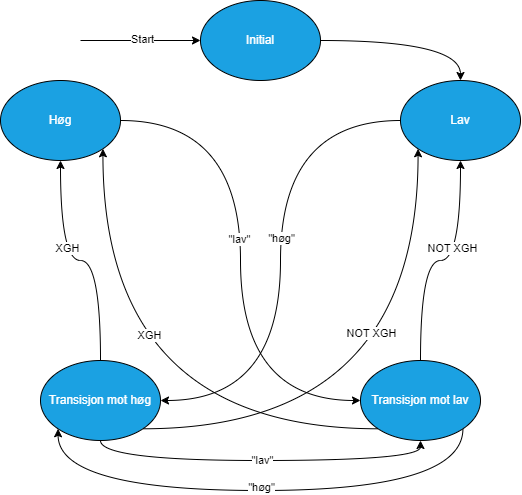
\includegraphics[scale=0.47]{Figurar/SBE.drawio.png}
    \caption{Prinsippskisse SBV tilstandsmaskin standard parameteroppsett}\label{fig:SBV tilstandsmaskin}
\end{figure}


Meir informasjon om blokka, inngangar, utgangar, og parameter er tilgjengeleg i vedlegg. (Vedlegg C.4)

\newpage


%\begin{figure}[htbp]
%    \centering
%    \begin{subfigure}[b]{0.45\textwidth}
%        \centering
%        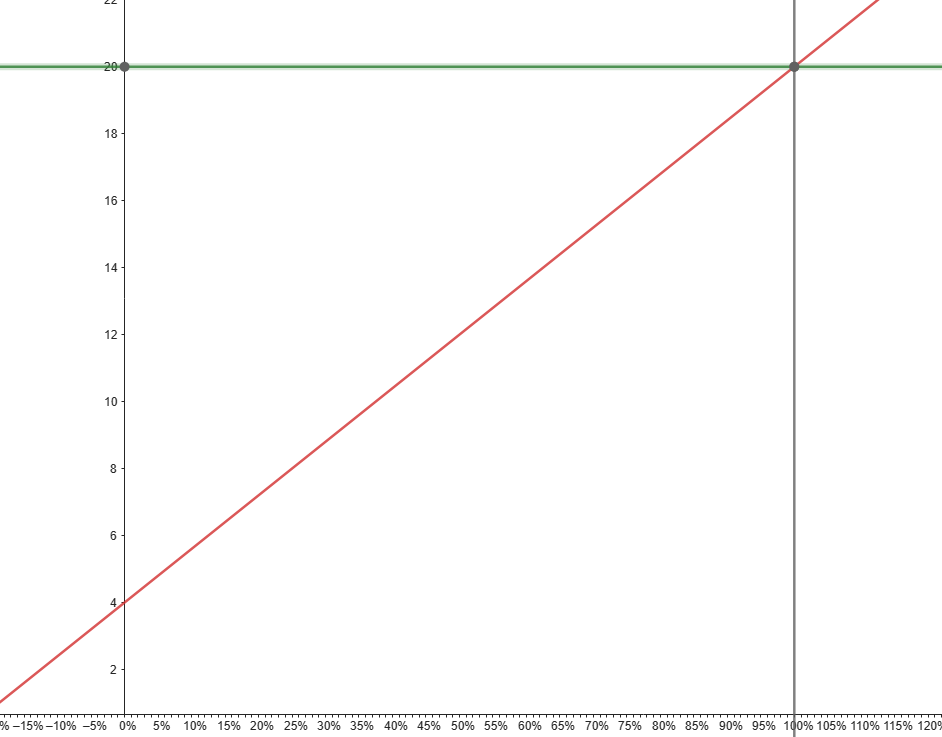
\includegraphics[width=1\textwidth]{Bilder/4_20mA_Scaling.png}
%        \caption{Skalering av mA mot prosent}\label{fig:Skalering av mA mot prosent}
%    \end{subfigure}
%    \hfill
%    \begin{subfigure}[b]{0.45\textwidth}
%        \centering
%        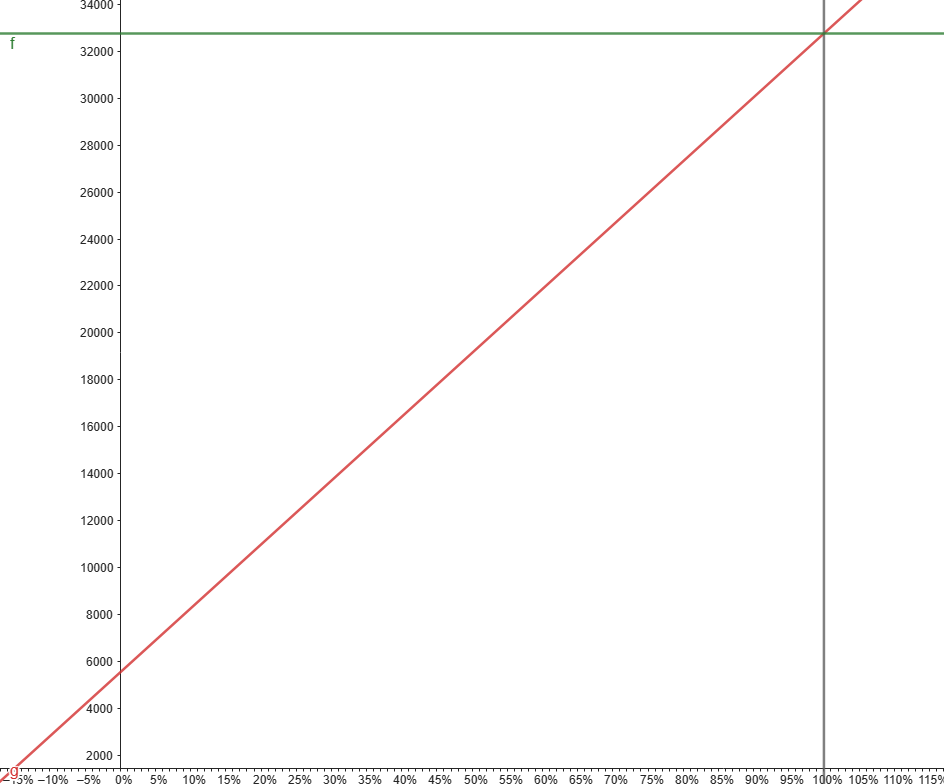
\includegraphics[width=0.95\textwidth]{Bilder/27327_prosent_Scaling.png}
%        \caption{Skalering av prosent til verdi}\label{fig:Skalering av prosent til verdi}
%    \end{subfigure}
%    \caption{Dei forskjellige skaleringane av inngangssignal}\label{fig:Skalering av prosent til verdi}
%\end{figure}


